\vfill
\begin{figure}[htb]\centering
  {%
    \setlength{\fboxsep}{7pt}%
    \setlength{\fboxrule}{1pt}%
    \fbox{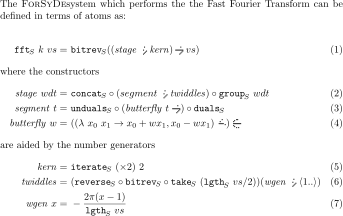
\includegraphics[width=.9\textwidth]{figs/example-forsyde-math}}
  }
\end{figure}
\lstinputlisting[firstline=4]{figs_src/example-forsyde-math.tex}
\vfill
\newpage

\section{The \texttt{forsyde-math} package}
\label{sec:forsyde-math-package}

This package provides a set of symbols and commands for writing equations. At the moment it covers only the formal notation associated with the \ForSyDeAtom\ framework. The package is imported using the command \texttt{\char`\\usepackage[math]\{forsyde\}} in the document preamble.

\subsection{Operator symbols}
\label{sec:fonts}

The \texttt{forsyde-math} package exports a set of symbols written in the \textsc{METAFONT} language (see \ref{sec:font-map}). These symbols are typed in using commands following the naming convention:

\begin{verbatim}
  \<name>               % inside a math environment
  \text<name>           % inside a text environment
\end{verbatim}

\noindent where the symbol name is from the table below\footnote{the symbol naming scheme reflects their semantics defined in the \ForSyDeAtom\ framework, as two acronyms: first one denoting the layer and the second one denoting the constructor}:\bookmark{operator symbols}

\def\makesymbolrow#1{{\tiny #1} & {\scriptsize #1} & {\footnotesize #1} & {\small #1} & {\normalsize #1} & {\large #1} & {\Large #1} & {\LARGE #1} & {\huge #1} & {\Huge #1}}
\begin{longtable} { c | c c c c c c c c c c }
  \toprule
  \texttt{<name>}  & \textbf{5pt} & \textbf{7pt} & \textbf{8pt} & \textbf{9pt} & \textbf{10pt} & \textbf{12pt} & \textbf{14.4pt} & \textbf{17.28pt} & \textbf{20.74pt} & \textbf{24.88pt} \\
  \midrule
  \texttt{BhFun} & \makesymbolrow{\textBhFun} \\
  \texttt{BhApp} & \makesymbolrow{\textBhApp} \\
  \texttt{BhDef} & \makesymbolrow{\textBhDef} \\
  \texttt{BhPhi} & \makesymbolrow{\textBhPhi} \\
  \texttt{BhDeg} & \makesymbolrow{\textBhDeg} \\
  \midrule
  \texttt{MocFun} & \makesymbolrow{\textMocFun} \\
  \texttt{MocApp} & \makesymbolrow{\textMocApp} \\
  \texttt{MocCmb} & \makesymbolrow{\textMocCmb} \\
  \texttt{MocPre} & \makesymbolrow{\textMocPre} \\
  \texttt{MocPhi} & \makesymbolrow{\textMocPhi} \\
  \texttt{MocDel} & \makesymbolrow{\textMocDel} \\
  \texttt{MocKern} & \makesymbolrow{\textMocKern} \\
  \midrule
  \texttt{SkelFrm} & \makesymbolrow{\textSkelFrm} \\
  \texttt{SkelPip} & \makesymbolrow{\textSkelPip} \\
  \texttt{SkelFun} & \makesymbolrow{\textSkelFun} \\
  \texttt{SkelApp} & \makesymbolrow{\textSkelApp} \\
  \texttt{SkelRed} & \makesymbolrow{\textSkelRed} \\
  \texttt{SkelRec} & \makesymbolrow{\textSkelRec} \\
  \bottomrule
\end{longtable}

\subsection{Math commands}
\label{sec:miscellaneous}

There are a couple of macros defined for math environments, mainly for convenience. They are listed below:\bookmark{math commands}
{\footnotesize
\begin{longtable} {  p{2.5cm} | c | c | p{6cm}  }
  \toprule
  \textbf{Command} & \textbf{Example} & \textbf{Result} & \textbf{Explanation}  \\
  \midrule
  \texttt{\string\id\{name\}} & \texttt{\$\string\id\{func\}\$} & $\id{func}$
  & wraps \texttt{name} as an identifier, rather than loose characters \\
  \texttt{\string\context\{ctx\}\{f\}} & \texttt{\$\string\context\{\string\Gamma\}\{f\}\$} & $ \context{\Gamma}{f} $
  & associates context \texttt{ctx} to function \texttt{f} \\
  \texttt{\string\Constructor} \texttt{\{name\}\{layer\}} & \texttt{\$\string\Constructor\{all\}\{T\}\$} & $ \Constructor{all}{T} $
  & generic infix name for constructor in a user-defined layer \\
  \texttt{\string\BhCons\{name\}} & \texttt{\$\string\BhCons\{default\}\$} & $ \BhCons{default} $
  & infix name for constructor in the \emph{behavior~layer} \\
  \texttt{\string\MocCons\{name\}} & \texttt{\$\string\MocCons\{mealy\}\$} & $ \MocCons{mealy} $
  & infix name for constructor in the \emph{MoC~layer} \\
  \texttt{\string\SkelCons\{name\}} & \texttt{\$\string\SkelCons\{mesh\}\$} & $ \SkelCons{mesh} $
  & infix name for constructor in the \emph{skeleton~layer} \\
  \texttt{\string\SkelVec\{exp\}} & \texttt{\$\string\SkelVec\{v\}\$} & $ \SkelVec{v} $
  & surrounds \texttt{exp} in vector type delimiters, associated with the \emph{skeleton layer} \\
  \bottomrule
\end{longtable}
}

\subsection{Font map}
\label{sec:font-map}



The \ForSyDeAtom\ operators from \ref{sec:fonts} have been created using \textsc{METAFONT} and have been bundled as a font family called \texttt{forsydeatom}. These fonts can be imported in accordance to the \LaTeXe\ standard. The math symbol font based on this font family is called \texttt{atomoperators} and it declares all symbols as binary operators.

In case you need to access the fonts directly (and not through the \texttt{forsyde-math} package), here is the mapping of the \texttt{forsydeatom} font family:
 
\begin{figure}[h]\centering
  \includegraphics[clip, trim=2.2cm 21cm 2cm 4cm, width=\textwidth]{figs/testfont}
\end{figure}

%%% Local Variables:
%%% TeX-command-default: "Make"
%%% mode: latex
%%% TeX-master: "../refman"
%%% End:
